\chapter{Example}

\begin{introduction}
\item 提要1
\item 提要2
\item 提要3
\item 提要4
\item 提要5
\end{introduction}

这是一个示例。

\section{环境}

\begin{theorem}{xxx定理}{label-for-this-theorem}
  这是一个定理。
\end{theorem}

\begin{example}
  这是一个例题。
\end{example}

\begin{definition}{xxx}{label-for-this-def}
  这是一个定义。
\end{definition}

\begin{lemma}{xxx引理}{label-for-this-lemma}
  这是一个引理。
\end{lemma}

\begin{proposition}{xxx命题}{label-for-this-prop}
  这是一个命题。
\end{proposition}

这是一个列表:

\begin{itemize}
  \item first thing
  \item second thing
    \begin{itemize}
      \item more of second thing
    \end{itemize}
  \item third thing
    \begin{enumerate}
      \item 可以是有序列表
      \item more of enumerate
    \end{enumerate}
\end{itemize}

这是一张图片:

\begin{figure}[hbt]
  \centering
  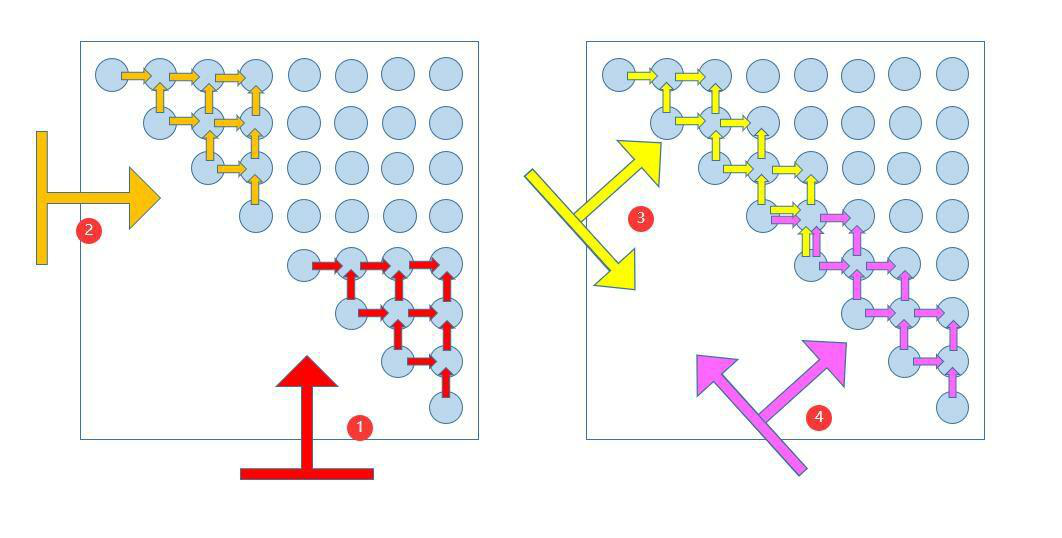
\includegraphics{image/dynamic-programming-1.png}
  \caption{这是一张图片}\label{fig:example}
\end{figure}

这是一段代码:

\begin{lstlisting}[language=Python, caption=Python example]
import numpy as np

def incmatrix(genl1,genl2):
    m = len(genl1)
    n = len(genl2)
    M = None #to become the incidence matrix
    VT = np.zeros((n*m,1), int)  #dummy variable

    #compute the bitwise xor matrix
    M1 = bitxormatrix(genl1)
    M2 = np.triu(bitxormatrix(genl2),1)

    for i in range(m-1):
        for j in range(i+1, m):
            [r,c] = np.where(M2 == M1[i,j])
            for k in range(len(r)):
                VT[(i)*n + r[k]] = 1;
                VT[(i)*n + c[k]] = 1;
                VT[(j)*n + r[k]] = 1;
                VT[(j)*n + c[k]] = 1;

                if M is None:
                    M = np.copy(VT)
                else:
                    M = np.concatenate((M, VT), 1)

                VT = np.zeros((n*m,1), int)

    return M
\end{lstlisting}

更多环境请见文档。

\section{引用}

\subsection{交叉引用}

引用定理~\ref{thm:label-for-this-theorem}。

\subsection{参考文献}

引用一个参考文献~\cite{cormen2009introduction}
